\setlength{\columnsep}{3pt}
\begin{flushleft}

\bigskip

\begin{itemize}
	\item \textbf{netstat}: Produce information related to network connections, routing tables, interface statistics etc.
	\newline
	Options with \textbf{netstat} command:
	\begin{itemize}
		\item \textbf{-r}: Display routing table
		\bigskip
		\begin{tcolorbox}[breakable,notitle,boxrule=0pt,colback=pink,colframe=pink]
			\color{black}
			\fontdimen2\font=1em
			Syntax: netstat -r
			\fontdimen2\font=4pt
		\end{tcolorbox}
		Eg:
		\begin{figure}[h!]
			\centering
			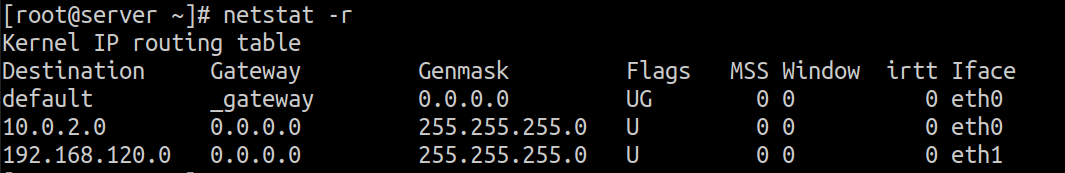
\includegraphics[scale=0.3]{content/chapter15/images/netstat_r.png}
			\caption{Sample output}
			\label{fig:output5}
		\end{figure}

		\item \textbf{-t}: Display \textbf{tcp} sockets
		\item \textbf{-u}: Display \textbf{udp} sockets
		\item \textbf{-l}: Display listening server sockets
		\item \textbf{-p}: Display PID/Program name for sockets
		\item \textbf{-n}: Don't resolve names
		\bigskip
		\begin{tcolorbox}[breakable,notitle,boxrule=0pt,colback=pink,colframe=pink]
			\color{black}
			\fontdimen2\font=1em
			Syntax: netstat -tulpn
			\fontdimen2\font=4pt
		\end{tcolorbox}
		Eg:
		\begin{figure}[h!]
			\centering
			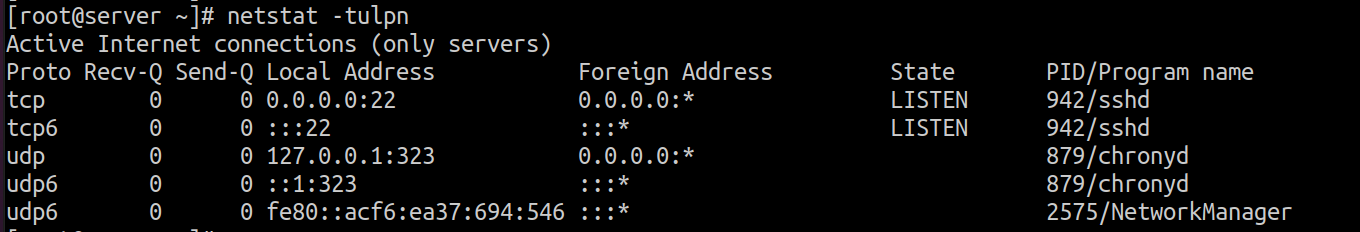
\includegraphics[scale=0.25]{content/chapter15/images/netstat_tulpn.png}
			\caption{Sample output}
			\label{fig:output6}
		\end{figure}
			
	\end{itemize}
	\newpage
	\item \textbf{tcpdump}: 
	\begin{itemize}
		\item Captures network package for future analysis.
	\end{itemize}
	\bigskip
	Option with \textbf{tcpdump} command:
	\begin{itemize}
		\item \textbf{-w}: Capture the network package in a file with \textbf{".pcap"} extension.
		\item \textbf{-i}: Interface name
		\item \textbf{-c}: Number of network packets to capture.
		\begin{tcolorbox}[breakable,notitle,boxrule=0pt,colback=pink,colframe=pink]
			\color{black}
			\fontdimen2\font=1em
			Syntax: tcpdump -c number\_of\_packets -w filename.pcap  -i interface\_name
			\fontdimen2\font=4pt
		\end{tcolorbox}
		Eg:
		\begin{figure}[h!]
			\centering
			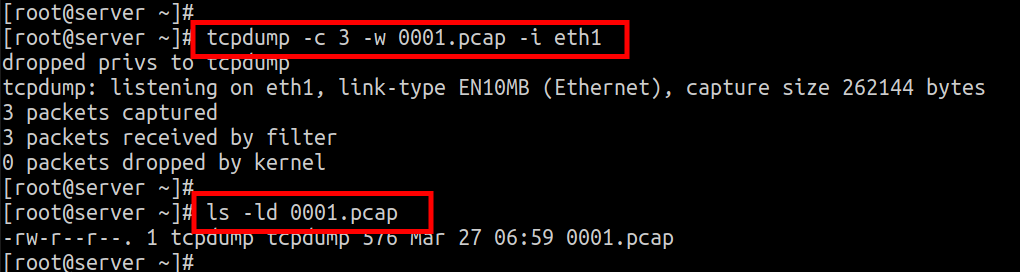
\includegraphics[scale=0.3]{content/chapter15/images/tcpdump_1.png}
			\caption{Sample output}
			\label{fig:output7}
		\end{figure}
	
		\item \textbf{-r}: Read \textbf{.pcap} file
		\begin{tcolorbox}[breakable,notitle,boxrule=0pt,colback=pink,colframe=pink]
			\color{black}
			\fontdimen2\font=1em
			Syntax: tcpdump -r filename.pcap
			\fontdimen2\font=4pt
		\end{tcolorbox}
		Eg:
		\begin{figure}[h!]
			\centering
			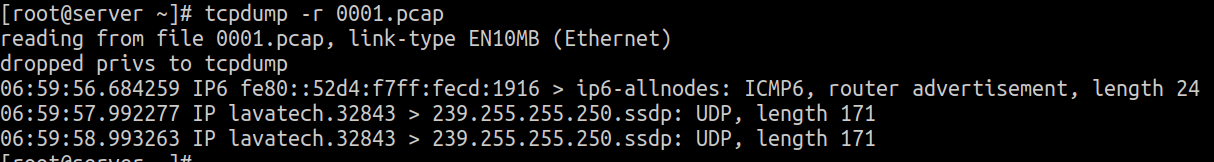
\includegraphics[scale=0.25]{content/chapter15/images/tcpdump_2.png}
			\caption{Sample output}
			\label{fig:output8}
		\end{figure}
		
		
		
	\end{itemize}


	
\end{itemize}

\end{flushleft}
\newpage


